\documentclass{standalone}
\usepackage{tikz}
\usetikzlibrary{patterns, positioning}


\begin{document}
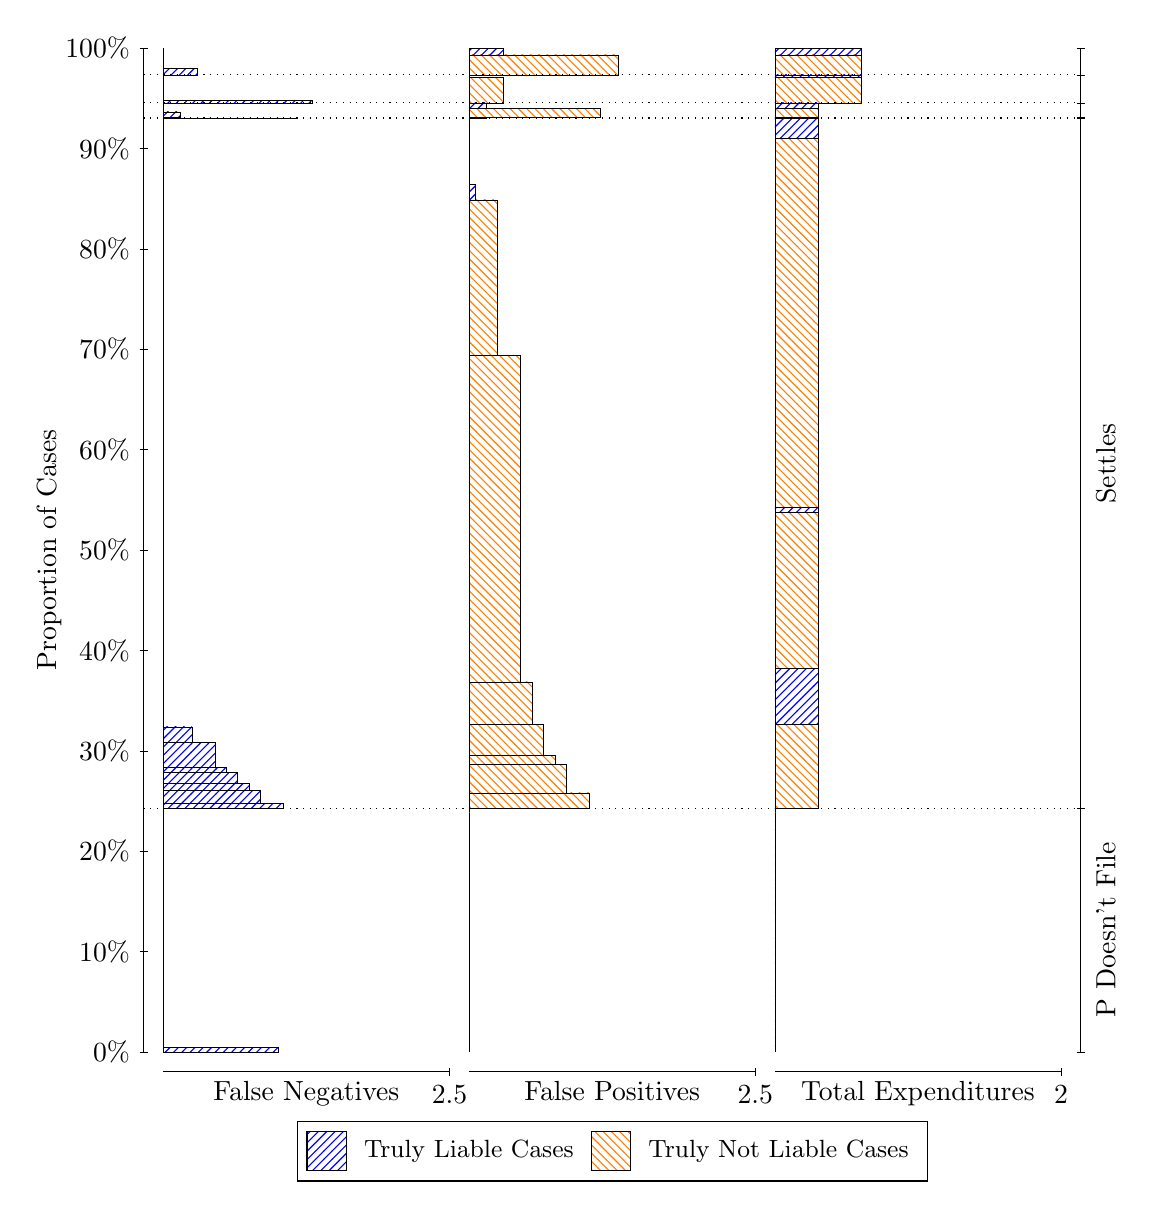
\begin{tikzpicture}
\draw[black, very thin] (1.5,1.75) -- (1.5,14.5);
\node[rotate=90, text=black, anchor=center] at (0.3, 8.125) {Proportion of Cases};
\draw[black, very thin] (1.45,1.75) -- (1.55,1.75);
\node[text=black, anchor=east] at (1.45, 1.75) {0\%};
\draw[black, very thin] (1.45,3.025) -- (1.55,3.025);
\node[text=black, anchor=east] at (1.45, 3.025) {10\%};
\draw[black, very thin] (1.45,4.3) -- (1.55,4.3);
\node[text=black, anchor=east] at (1.45, 4.3) {20\%};
\draw[black, very thin] (1.45,5.575) -- (1.55,5.575);
\node[text=black, anchor=east] at (1.45, 5.575) {30\%};
\draw[black, very thin] (1.45,6.85) -- (1.55,6.85);
\node[text=black, anchor=east] at (1.45, 6.85) {40\%};
\draw[black, very thin] (1.45,8.125) -- (1.55,8.125);
\node[text=black, anchor=east] at (1.45, 8.125) {50\%};
\draw[black, very thin] (1.45,9.4) -- (1.55,9.4);
\node[text=black, anchor=east] at (1.45, 9.4) {60\%};
\draw[black, very thin] (1.45,10.675) -- (1.55,10.675);
\node[text=black, anchor=east] at (1.45, 10.675) {70\%};
\draw[black, very thin] (1.45,11.95) -- (1.55,11.95);
\node[text=black, anchor=east] at (1.45, 11.95) {80\%};
\draw[black, very thin] (1.45,13.225) -- (1.55,13.225);
\node[text=black, anchor=east] at (1.45, 13.225) {90\%};
\draw[black, very thin] (1.45,14.5) -- (1.55,14.5);
\node[text=black, anchor=east] at (1.45, 14.5) {100\%};

\draw[black, very thin] (13.4,1.75) -- (13.4,14.5);
\draw[black, very thin] (13.35,1.75) -- (13.45,1.75);
\node[anchor=west] at (13.35, 1.75) {};
\draw[black, very thin] (13.35,4.8475) -- (13.45,4.8475);
\node[anchor=west] at (13.35, 4.8475) {};
\draw[black, very thin] (13.35,13.602) -- (13.45,13.602);
\node[anchor=west] at (13.35, 13.602) {};
\draw[black, very thin] (13.35,13.615) -- (13.45,13.615);
\node[anchor=west] at (13.35, 13.615) {};
\draw[black, very thin] (13.35,13.803) -- (13.45,13.803);
\node[anchor=west] at (13.35, 13.803) {};
\draw[black, very thin] (13.35,14.159) -- (13.45,14.159);
\node[anchor=west] at (13.35, 14.159) {};
\draw[black, very thin] (13.35,14.5) -- (13.45,14.5);
\node[anchor=west] at (13.35, 14.5) {};

\draw[black, very thin, pattern color=blue, pattern=north east lines] (1.75,1.75) rectangle (3.2033,1.8049);
\draw[black, very thin, pattern color=orange, pattern=north west lines] (1.75,1.8049) rectangle (1.75,4.8475);
\draw[black, very thin, pattern color=blue, pattern=north east lines] (1.75,4.8475) rectangle (3.276,4.911);
\draw[black, very thin, pattern color=blue, pattern=north east lines] (1.75,4.911) rectangle (2.9853,5.0736);
\draw[black, very thin, pattern color=blue, pattern=north east lines] (1.75,5.0736) rectangle (2.84,5.1636);
\draw[black, very thin, pattern color=blue, pattern=north east lines] (1.75,5.1636) rectangle (2.6947,5.2972);
\draw[black, very thin, pattern color=blue, pattern=north east lines] (1.75,5.2972) rectangle (2.5493,5.3653);
\draw[black, very thin, pattern color=blue, pattern=north east lines] (1.75,5.3653) rectangle (2.404,5.6781);
\draw[black, very thin, pattern color=blue, pattern=north east lines] (1.75,5.6781) rectangle (2.1133,5.8788);
\draw[black, very thin, pattern color=orange, pattern=north west lines] (1.75,5.8788) rectangle (1.75,13.602);
\draw[black, very thin, pattern color=blue, pattern=north east lines] (1.75,13.602) rectangle (3.4213,13.603);
\draw[black, very thin, pattern color=orange, pattern=north west lines] (1.75,13.603) rectangle (1.75,13.615);
\draw[black, very thin, pattern color=blue, pattern=north east lines] (1.75,13.615) rectangle (1.968,13.688);
\draw[black, very thin, pattern color=orange, pattern=north west lines] (1.75,13.688) rectangle (1.75,13.803);
\draw[black, very thin, pattern color=blue, pattern=north east lines] (1.75,13.803) rectangle (3.6393,13.831);
\draw[black, very thin, pattern color=orange, pattern=north west lines] (1.75,13.831) rectangle (1.75,14.159);
\draw[black, very thin, pattern color=blue, pattern=north east lines] (1.75,14.159) rectangle (2.186,14.246);
\draw[black, very thin, pattern color=orange, pattern=north west lines] (1.75,14.246) rectangle (1.75,14.5);
\draw[black, very thin, pattern color=orange, pattern=north west lines] (5.6333,1.75) rectangle (5.6333,4.7925);
\draw[black, very thin, pattern color=blue, pattern=north east lines] (5.6333,4.7925) rectangle (5.6333,4.8475);
\draw[black, very thin, pattern color=orange, pattern=north west lines] (5.6333,4.8475) rectangle (7.1593,5.0414);
\draw[black, very thin, pattern color=orange, pattern=north west lines] (5.6333,5.0414) rectangle (6.8687,5.401);
\draw[black, very thin, pattern color=orange, pattern=north west lines] (5.6333,5.401) rectangle (6.7233,5.5129);
\draw[black, very thin, pattern color=orange, pattern=north west lines] (5.6333,5.5129) rectangle (6.578,5.9111);
\draw[black, very thin, pattern color=orange, pattern=north west lines] (5.6333,5.9111) rectangle (6.4327,6.4489);
\draw[black, very thin, pattern color=orange, pattern=north west lines] (5.6333,6.4489) rectangle (6.2873,10.592);
\draw[black, very thin, pattern color=orange, pattern=north west lines] (5.6333,10.592) rectangle (5.9967,12.571);
\draw[black, very thin, pattern color=blue, pattern=north east lines] (5.6333,12.571) rectangle (5.706,12.771);
\draw[black, very thin, pattern color=blue, pattern=north east lines] (5.6333,12.771) rectangle (5.6333,13.602);
\draw[black, very thin, pattern color=orange, pattern=north west lines] (5.6333,13.602) rectangle (5.8513,13.615);
\draw[black, very thin, pattern color=blue, pattern=north east lines] (5.6333,13.615) rectangle (5.6333,13.615);
\draw[black, very thin, pattern color=orange, pattern=north west lines] (5.6333,13.615) rectangle (7.3047,13.729);
\draw[black, very thin, pattern color=blue, pattern=north east lines] (5.6333,13.729) rectangle (5.8513,13.803);
\draw[black, very thin, pattern color=orange, pattern=north west lines] (5.6333,13.803) rectangle (6.0693,14.131);
\draw[black, very thin, pattern color=blue, pattern=north east lines] (5.6333,14.131) rectangle (5.6333,14.159);
\draw[black, very thin, pattern color=orange, pattern=north west lines] (5.6333,14.159) rectangle (7.5227,14.413);
\draw[black, very thin, pattern color=blue, pattern=north east lines] (5.6333,14.413) rectangle (6.0693,14.5);
\draw[black, very thin, pattern color=orange, pattern=north west lines] (9.5167,1.75) rectangle (9.5167,4.7925);
\draw[black, very thin, pattern color=blue, pattern=north east lines] (9.5167,4.7925) rectangle (9.5167,4.8475);
\draw[black, very thin, pattern color=orange, pattern=north west lines] (9.5167,4.8475) rectangle (10.062,5.9111);
\draw[black, very thin, pattern color=blue, pattern=north east lines] (9.5167,5.9111) rectangle (10.062,6.6264);
\draw[black, very thin, pattern color=orange, pattern=north west lines] (9.5167,6.6264) rectangle (10.062,8.6046);
\draw[black, very thin, pattern color=blue, pattern=north east lines] (9.5167,8.6046) rectangle (10.062,8.6682);
\draw[black, very thin, pattern color=orange, pattern=north west lines] (9.5167,8.6682) rectangle (10.062,13.349);
\draw[black, very thin, pattern color=blue, pattern=north east lines] (9.5167,13.349) rectangle (10.062,13.602);
\draw[black, very thin, pattern color=orange, pattern=north west lines] (9.5167,13.602) rectangle (10.062,13.615);
\draw[black, very thin, pattern color=blue, pattern=north east lines] (9.5167,13.615) rectangle (10.062,13.615);
\draw[black, very thin, pattern color=orange, pattern=north west lines] (9.5167,13.615) rectangle (10.062,13.729);
\draw[black, very thin, pattern color=blue, pattern=north east lines] (9.5167,13.729) rectangle (10.062,13.803);
\draw[black, very thin, pattern color=orange, pattern=north west lines] (9.5167,13.803) rectangle (10.607,14.131);
\draw[black, very thin, pattern color=blue, pattern=north east lines] (9.5167,14.131) rectangle (10.607,14.159);
\draw[black, very thin, pattern color=orange, pattern=north west lines] (9.5167,14.159) rectangle (10.607,14.413);
\draw[black, very thin, pattern color=blue, pattern=north east lines] (9.5167,14.413) rectangle (10.607,14.5);
\draw[black, dotted] (1.5,4.8475) -- (13.4,4.8475);
\draw[black, dotted] (1.5,13.602) -- (13.4,13.602);
\draw[black, dotted] (1.5,13.615) -- (13.4,13.615);
\draw[black, dotted] (1.5,13.803) -- (13.4,13.803);
\draw[black, dotted] (1.5,14.159) -- (13.4,14.159);
\draw[black, very thin] (1.75,1.5) -- (5.3833,1.5);
\node[text=black, anchor=north] at (3.5667, 1.5) {False Negatives};
\draw[black, very thin] (5.3833,1.45) -- (5.3833,1.55);
\node[text=black, anchor=north] at (5.3833, 1.45) {2.5};

\draw[black, very thin] (5.6333,1.5) -- (9.2667,1.5);
\node[text=black, anchor=north] at (7.45, 1.5) {False Positives};
\draw[black, very thin] (9.2667,1.45) -- (9.2667,1.55);
\node[text=black, anchor=north] at (9.2667, 1.45) {2.5};

\draw[black, very thin] (9.5167,1.5) -- (13.15,1.5);
\node[text=black, anchor=north] at (11.333, 1.5) {Total Expenditures};
\draw[black, very thin] (13.15,1.45) -- (13.15,1.55);
\node[text=black, anchor=north] at (13.15, 1.45) {2};

\node[text=black, centered, rotate=90] at (13.72, 3.2987) {P Doesn't File};
\node[text=black, centered, rotate=90] at (13.72, 9.2247) {Settles};





\draw (7.449999999999999,1.5) node[draw=none] (baseCoordinate) {};
\begin{scope}[align=center]
        \matrix[scale=0.5, draw=black, below=0.5cm of baseCoordinate, nodes={draw}, column sep=0.1cm]{
            \node[rectangle, draw, minimum width=0.5cm, minimum height=0.5cm, pattern color=blue, pattern=north east lines] {}; &
            \node[draw=none, font=\small, text=black] (B) {Truly Liable Cases}; &
            \node[rectangle, draw, minimum width=0.5cm, minimum height=0.5cm, pattern color=orange, pattern=north west lines] {}; &
            \node[draw=none, font=\small, text=black] (B) {Truly Not Liable Cases}; \\
            };
\end{scope}

\end{tikzpicture}
\end{document}